% ============================================================ two electrons in two orbitals + the sign error
\section{Two electrons, two orbitals}

\begin{frame}{Six ways to place two electrons}{Figure 1 of the review, rebuilt}
  \centering
  \begin{tikzpicture}[scale=1.15]
    \foreach \lab/\x/\ms in {i/0/0,ii/1.6/0,iii/3.2/0,iv/4.8/0,v/6.4/{+1},vi/8.0/{-1}}{
      \node[font=\small\itshape,text=noirgold] at (\x,1.85) {\lab};
      \draw[level] (\x-0.4,0) -- (\x+0.4,0);
      \draw[level] (\x-0.4,1.1) -- (\x+0.4,1.1);
      \node[font=\small,text=noirmuted] at (\x,-0.7) {$M_S=\ms$};
    }
    \node[font=\small,text=noirfg] at (-0.95,0) {$\pa$};
    \node[font=\small,text=noirfg] at (-0.95,1.1) {$\pb$};
    \onslide<2->{\elup{0}{0}\eldn{0}{0}}
    \onslide<3->{\elup{1.6}{1.1}\eldn{1.6}{1.1}}
    \onslide<4->{\elup{3.2}{0}\eldn{3.2}{1.1}}
    \onslide<5->{\eldn{4.8}{0}\elup{4.8}{1.1}}
    \onslide<6->{\elup{6.4}{0}\elup{6.4}{1.1}}
    \onslide<7->{\eldn{8.0}{0}\eldn{8.0}{1.1}}
    \onslide<8->{
      \draw[decorate,decoration={brace,amplitude=5pt,mirror},noirblue] (-0.45,-1.0) -- (1.95,-1.0)
        node[midway,below=6pt,font=\scriptsize,text=noirblue]{closed shells};
      \draw[decorate,decoration={brace,amplitude=5pt,mirror},noirviolet] (2.75,-1.0) -- (5.25,-1.0)
        node[midway,below=6pt,font=\scriptsize,text=noirviolet]{open shell, $M_S=0$};
      \draw[decorate,decoration={brace,amplitude=5pt,mirror},noirrose] (5.95,-1.0) -- (8.45,-1.0)
        node[midway,below=6pt,font=\scriptsize,text=noirrose]{high spin};}
  \end{tikzpicture}
  \vskip0.1cm
  \onslide<8->{\small four spin orbitals $\pa\alpha,\pa\beta,\pb\alpha,\pb\beta$; choose 2 of 4 \;$\Rightarrow$\; $\binom42=6$ determinants}
  \symbolstrip{$\pa,\pb$: the two spatial orbitals (real, orthonormal), e.g.\ the two frontier orbitals of a diradical \quad
    \textcolor{noirrose}{$\uparrow$}/\textcolor{noirblue}{$\downarrow$}: electron with spin $\alpha$/$\beta$ \quad
    $M_S$: total $S_z$ $=$ sum of $+\tfrac12$ per $\uparrow$ and $-\tfrac12$ per $\downarrow$}
\end{frame}

\begin{frame}{The paper's Figure 1}
  \begin{columns}[c]
    \column{0.55\textwidth}
    \centering
    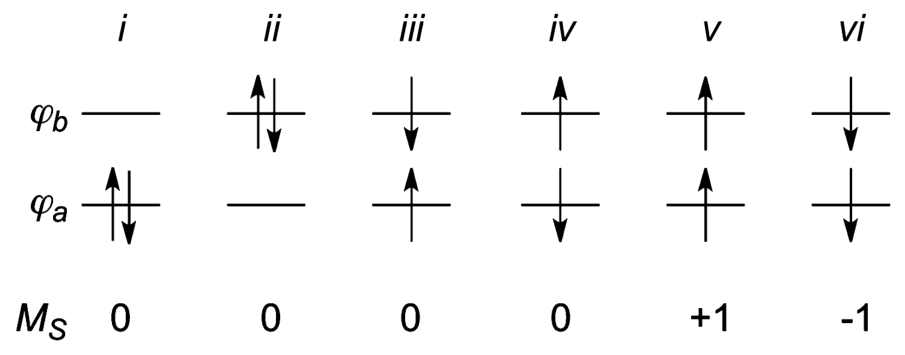
\includegraphics[width=\linewidth]{fig01_two_electron_determinants.png}
    \column{0.42\textwidth}
    \begin{paperclaim}
      ``Various arrangements (determinants) of two electrons in two molecular orbitals and the corresponding
      values of the secondary spin quantum number.'' (p.\ 441)
    \end{paperclaim}
    \onslide<2->{\small\cgreen{Matches our reconstruction.} Now write each one out.}
  \end{columns}
  \symbolstrip{``secondary spin quantum number'' $=M_S$, the projection of the total spin on the $z$ axis}
\end{frame}

\begin{frame}{Writing the determinants out}
  \small
  shorthand: \quad $\ccyan{A}\equiv\pa(1)\pb(2)$ \cmuted{(electron 1 in $\pa$, 2 in $\pb$)},\qquad
  $\crose{B}\equiv\pb(1)\pa(2)$ \cmuted{(swapped)}
  \vskip0.1cm
  \begin{center}
  \renewcommand{\arraystretch}{1.2}
  \begin{tabular}{@{}l l l@{}}
    \toprule
    & spin orbitals $\chi_1,\chi_2$ & $D=\chi_1(1)\chi_2(2)-\chi_2(1)\chi_1(2)$\\
    \midrule
    i   & $\pa\alpha,\ \pa\beta$ & $\pa(1)\pa(2)\,(\alpha_1\beta_2-\beta_1\alpha_2)$\\
    ii  & $\pb\alpha,\ \pb\beta$ & $\pb(1)\pb(2)\,(\alpha_1\beta_2-\beta_1\alpha_2)$\\
    \onslide<2->{iii} & \onslide<2->{$\pa\alpha,\ \pb\beta$} & \onslide<2->{$\ccyan{A}\,\alpha_1\beta_2-\crose{B}\,\beta_1\alpha_2$}\\
    \onslide<3->{iv}  & \onslide<3->{$\pa\beta,\ \pb\alpha$} & \onslide<3->{$\ccyan{A}\,\beta_1\alpha_2-\crose{B}\,\alpha_1\beta_2$}\\
    \onslide<4->{v}   & \onslide<4->{$\pa\alpha,\ \pb\alpha$} & \onslide<4->{$(\ccyan{A}-\crose{B})\,\alpha_1\alpha_2$}\\
    \onslide<4->{vi}  & \onslide<4->{$\pa\beta,\ \pb\beta$} & \onslide<4->{$(\ccyan{A}-\crose{B})\,\beta_1\beta_2$}\\
    \bottomrule
  \end{tabular}
  \end{center}
  \onslide<2->{\cmuted{e.g.\ iii: }$\chi_1=\pa\alpha,\ \chi_2=\pb\beta$:\quad
  $\pa(1)\alpha_1\,\pb(2)\beta_2-\pb(1)\beta_1\,\pa(2)\alpha_2$}
  \explain<2->{in each product the spatial part and the spin part of the same electron travel together}
  \symbolstrip{$D_{\text{X}}$: \emph{unnormalised} determinant of row X (its normalised form is $\tfrac1{\sqrt2}D$) \quad
    $\pa(1)$: orbital $\pa$ evaluated at electron 1's position $\mathbf r_1$ \quad $\alpha_1\beta_2$: electron 1 up, electron 2 down}
\end{frame}

\begin{frame}{$M_S=\pm1$: one determinant each}
  \begin{align*}
    \tfrac1{\sqrt2}D_{\text v}&=\underbrace{\tfrac1{\sqrt2}\bigl[\pa(1)\pb(2)-\pb(1)\pa(2)\bigr]}_{\text{antisymmetric space}}\;
      \underbrace{\alpha_1\alpha_2}_{\Theta_{1,+1}} &&\why{row v: $(A-B)\,\alpha_1\alpha_2$}\\
    \uncover<2->{\tfrac1{\sqrt2}D_{\text{vi}}}&\uncover<2->{=\tfrac1{\sqrt2}\bigl[\pa(1)\pb(2)-\pb(1)\pa(2)\bigr]\;\beta_1\beta_2}
      &&\uncover<2->{\why{same space, both spins down}}
  \end{align*}
  \onslide<3->{
  \begin{paperclaim}
    ``$^3\Psi(M_s=+1)=\tfrac1{\sqrt2}[\pa(1)\pb(2)-\pb(1)\pa(2)][\alpha_1\alpha_2]$'' \dots\ ``i.e., they can be
    represented as single determinants v and vi'' (p.\ 441; $M_s=-1$ analogous with $\beta_1\beta_2$)
  \end{paperclaim}}
  \onslide<4->{\centering\okpill\quad\small exactly right: the high-spin triplet components are \cgold{single-reference}.\par}
  \symbolstrip{$^3\Psi$: triplet ($2S+1=3$) \quad one determinant already factorises into (space)$\times$(spin of definite $S$) \quad
    $\tfrac1{\sqrt2}$ normalises $A-B$, since $\braket{A-B}{A-B}=2$}
\end{frame}

\begin{frame}{$M_S=0$: iii and iv are not spin eigenfunctions}
  \begin{columns}[c]
    \column{0.55\textwidth}
    \[
      D_{\text{iii}}=\ccyan{A}\,\underbrace{\alpha_1\beta_2}_{\text{not }\Theta}-\crose{B}\,\underbrace{\beta_1\alpha_2}_{\text{not }\Theta}
    \]
    \onslide<2->{From the spin slides:
    \[
      \hat S^2\alpha_1\beta_2=\alpha_1\beta_2+\beta_1\alpha_2\neq\lambda\,\alpha_1\beta_2
    \]}
    \onslide<3->{\small so $D_{\text{iii}}$ is half singlet, half triplet. \\
      \cgold{Only combinations of iii and iv have definite spin.}}
    \column{0.4\textwidth}
    \centering
    \begin{tikzpicture}[scale=1.2]
      \draw[level] (-0.4,0) -- (0.4,0); \draw[level] (-0.4,1.1) -- (0.4,1.1);
      \elup{0}{0}\eldn{0}{1.1}
      \node[font=\small] at (0.95,0.55) {$\pm$};
      \draw[level] (1.5,0) -- (2.3,0); \draw[level] (1.5,1.1) -- (2.3,1.1);
      \eldn{1.9}{0}\elup{1.9}{1.1}
      \node[font=\scriptsize,text=noirmuted] at (0,-0.4) {iii};
      \node[font=\scriptsize,text=noirmuted] at (1.9,-0.4) {iv};
      \onslide<3->{\node[font=\scriptsize,text=noirgold] at (0.95,-0.95) {$+$ or $-$ \ ?};}
    \end{tikzpicture}
  \end{columns}
  \explain<3->{``half and half'': $\alpha_1\beta_2=\tfrac1{\sqrt2}(\Theta_{1,0}+\Theta_{0,0})$, so $\braket{\hat S^2}=\tfrac12\cdot2+\tfrac12\cdot0=1$ (T1b measures exactly 1)}
  \symbolstrip{$\Theta$: a spin eigenfunction (definite $S$) \quad $\lambda$: would-be eigenvalue \quad
    eigenfunction: $\hat S^2f=\lambda f$ with the \emph{same} $f$ on both sides}
\end{frame}

\begin{frame}{The sum $D_{\text{iii}}+D_{\text{iv}}$, every term tracked}
  \begin{align*}
    D_{\text{iii}}+D_{\text{iv}}
      &=\ccyan{A}\,\alpha_1\beta_2-\crose{B}\,\beta_1\alpha_2+\ccyan{A}\,\beta_1\alpha_2-\crose{B}\,\alpha_1\beta_2
        &&\why{rows iii, iv}\\
      &\uncover<2->{=\ccyan{A}\,(\alpha_1\beta_2+\beta_1\alpha_2)-\crose{B}\,(\beta_1\alpha_2+\alpha_1\beta_2)}
        &&\uncover<2->{\why{collect $A$, $B$}}\\
      &\uncover<3->{=(\ccyan{A}-\crose{B})\,(\alpha_1\beta_2+\beta_1\alpha_2)}
        &&\uncover<3->{\why{same bracket}}\\
      &\uncover<4->{=\underbrace{\bigl[\pa(1)\pb(2)-\pb(1)\pa(2)\bigr]}_{\text{antisymmetric space}}
        \underbrace{(\alpha_1\beta_2+\beta_1\alpha_2)}_{\sqrt2\,\Theta_{1,0}}}
        &&\uncover<4->{\why{put $A$, $B$ back}}
  \end{align*}
  \onslide<5->{
  \begin{keyresult}
    antisymmetric space $\times$ symmetric spin: the \emph{sum} is the $M_S=0$ \crose{triplet}.
  \end{keyresult}}
  \symbolstrip{$A=\pa(1)\pb(2)$, $B=\pb(1)\pa(2)$ \quad $A-B$ changes sign under $1\leftrightarrow2$ (antisymmetric) \quad
    $\Theta_{1,0}=\tfrac1{\sqrt2}(\alpha_1\beta_2+\beta_1\alpha_2)$: triplet, $M_S=0$}
\end{frame}

\begin{frame}{The difference $D_{\text{iv}}-D_{\text{iii}}$}
  \begin{align*}
    D_{\text{iv}}-D_{\text{iii}}
      &=\ccyan{A}\,\beta_1\alpha_2-\crose{B}\,\alpha_1\beta_2-\ccyan{A}\,\alpha_1\beta_2+\crose{B}\,\beta_1\alpha_2
        &&\why{iv minus iii}\\
      &\uncover<2->{=\ccyan{A}\,(\beta_1\alpha_2-\alpha_1\beta_2)+\crose{B}\,(\beta_1\alpha_2-\alpha_1\beta_2)}
        &&\uncover<2->{\why{collect $A$ and $B$}}\\
      &\uncover<3->{=(\ccyan{A}+\crose{B})\,(\beta_1\alpha_2-\alpha_1\beta_2)}
        &&\uncover<3->{\why{common bracket}}\\
      &\uncover<4->{=\underbrace{\bigl[\pa(1)\pb(2)+\pb(1)\pa(2)\bigr]}_{\text{symmetric space}}
        \underbrace{(\beta_1\alpha_2-\alpha_1\beta_2)}_{-\sqrt2\,\Theta_{0,0}}}
        &&\uncover<4->{\why{put $A$, $B$ back}}
  \end{align*}
  \onslide<5->{
  \begin{keyresult}
    symmetric space $\times$ antisymmetric spin: the \emph{difference} is the \cblue{open-shell singlet}.
  \end{keyresult}}
  \symbolstrip{$A+B$ is unchanged under $1\leftrightarrow2$ (symmetric) \quad $\Theta_{0,0}=\tfrac1{\sqrt2}(\alpha_1\beta_2-\beta_1\alpha_2)$: singlet;
    $\beta_1\alpha_2-\alpha_1\beta_2=-\sqrt2\,\Theta_{0,0}$ (overall sign of a state is irrelevant)}
\end{frame}

\begin{frame}{Normalisation}
  \begin{columns}[c]
    \column{0.66\textwidth}
    {\begin{align*}
      \braket{A\pm B}{A\pm B}&=\braket AA+\braket BB\pm2\braket AB &&\why{expand}\\
      \uncover<2->{\braket AA}&\uncover<2->{=\braket{\pa}{\pa}\braket{\pb}{\pb}=1} &&\uncover<2->{\why{split the integrals}}\\
      \uncover<3->{\braket AB}&\uncover<3->{=\braket{\pa}{\pb}\braket{\pb}{\pa}=\canc<4->{0\cdot0}=0} &&\uncover<3->{\why{orthogonal}}\\
      \uncover<5->{\Rightarrow\ \braket{A\pm B}{A\pm B}}&\uncover<5->{=2} &&
    \end{align*}}
    \onslide<6->{each combination needs $\dfrac1{\sqrt2}\cdot\dfrac1{\sqrt2}=\dfrac12$}
    \explain<6->{spin part likewise: $\|\alpha_1\beta_2\pm\beta_1\alpha_2\|^2=2$; one $\tfrac1{\sqrt2}$ for space, one for spin}
    \column{0.31\textwidth}
    \onslide<7->{
    \begin{keyresult}
      \vskip-0.6em
      {\begin{align*}
        ^3\Psi_0&=\tfrac12(D_{\text{iii}}+D_{\text{iv}})\\
        ^1\Psi_{\OSS}&=\tfrac12(D_{\text{iv}}-D_{\text{iii}})
      \end{align*}}
    \end{keyresult}}
  \end{columns}
  \symbolstrip{$\braket fg=\iint f^*g\,\dd\mathbf r_1\dd\mathbf r_2$ (spin sums for spin functions) \quad $\|f\|^2=\braket ff$ \quad
    $^3\Psi_0$: triplet, $M_S=0$ \quad $^1\Psi_{\OSS}$: open-shell singlet}
\end{frame}

\begin{frame}{Now read the paper}{spot the difference}
  \centering
  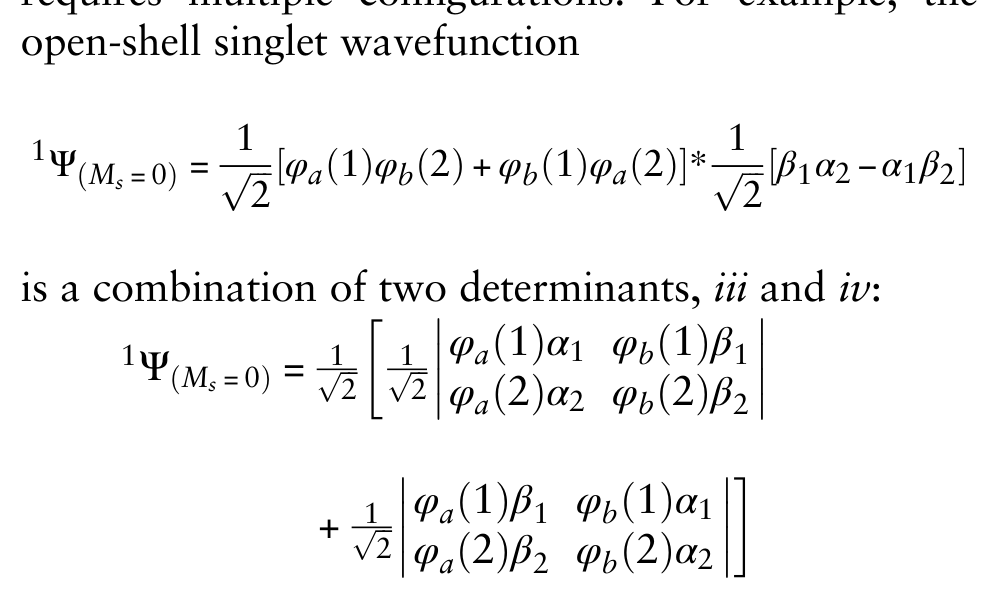
\includegraphics[height=0.56\textheight]{screenshots/sign_error_raw.png}
  \vskip0.1cm
  \onslide<2->{\small Line 1 (product form) \ldots\ then ``is a combination of two determinants, iii and iv:''}
  \symbolstrip{the paper writes each determinant with rows $=$ electrons 1, 2 and columns $=$ spin orbitals, exactly our $D_{\text{iii}}$ and
    $D_{\text{iv}}$; its prefactor $\tfrac1{\sqrt2}\cdot\tfrac1{\sqrt2}=\tfrac12$ matches ours}
\end{frame}

\begin{frame}{Spotted it}
  \begin{columns}[c]
    \column{0.6\textwidth}
    \centering
    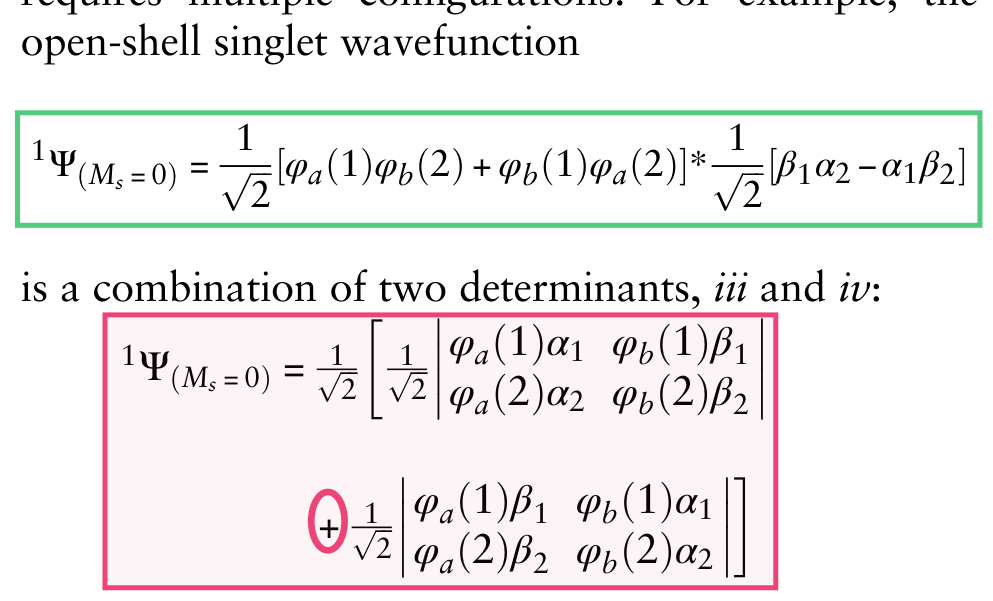
\includegraphics[width=\linewidth]{screenshots/sign_error_marked.png}
    \column{0.38\textwidth}
    \begin{itemize}
      \item<2-> \cgreen{green}: product form, symmetric space $\times$ antisymmetric spin \hfill\okpill
      \item<3-> \crose{rose}: $\tfrac12(D_{\text{iii}}\ \crose{+}\ D_{\text{iv}})$ is what we just proved to be the
            \crose{triplet} \hfill\badpill
    \end{itemize}
    \onslide<4->{
    \begin{erratum}
      should read \;$\tfrac12(D_{\text{iv}}\ \cgreen{-}\ D_{\text{iii}})$
    \end{erratum}}
  \end{columns}
  \symbolstrip{the two lines contradict each other: line 1 (green) equals $\tfrac12(D_{\text{iv}}-D_{\text{iii}})$; line 2 (rose) does not}
\end{frame}

\begin{frame}{Fluctuating multiplicity, live in print}
  \centering
  \begin{tikzpicture}
    \node[font=\noircalli\fontsize{60}{60}\selectfont,text=noirrose] (p) at (0,0) {$+$};
    \node[font=\noircalli\fontsize{60}{60}\selectfont,text=noirgreen] (m) at (5,0) {$-$};
    \draw[-{Stealth[length=7pt]},noirgold,line width=1pt] (0.9,0) -- node[above,font=\small]{one character} (4.1,0);
    \node[font=\small,text=noirrose] at (0,-1.1) {$S=1$};
    \node[font=\small,text=noirgreen] at (5,-1.1) {$S=0$};
  \end{tikzpicture}
  \vskip0.3cm
  \onslide<2->{\large The section is titled \emph{``Fluctuating ground-state multiplicity''}\ldots}
  \vskip0.2cm
  \onslide<3->{\large \ldots and between two lines the open-shell singlet \cgold{fluctuates into a triplet}.}
  \vskip0.2cm
  \onslide<4->{\small\cmuted{(It survived peer review and typesetting. Two referees with parallel spins, presumably:
    the Fermi hole kept them from ever meeting the error.)}}
\end{frame}

\begin{frame}[fragile]{Checked three ways: SymPy, $\hat S^2$, Lean}
  \begin{columns}[T]
    \column{0.49\textwidth}
    \cgold{SymPy} (T1): symbolic expansion
\begin{minted}[fontsize=\tiny]{text}
3Psi(0)  = (iii+iv)/2           : True
1Psi_OSS = (iv-iii)/2           : True
paper's (iii+iv)/2 == OSS ?     : False
\end{minted}
    \onslide<2->{\cgold{$\hat S^2$ as an operator} (T1b): the paper's matrices on a grid}
\begin{onlyenv}<2->
\begin{minted}[fontsize=\tiny]{text}
paper:   (1/2)(|iii| + |iv|)  <S^2> = +2.000000  TRIPLET
correct: (1/2)(|iv| - |iii|)  <S^2> = +0.000000  SINGLET
paper's product form (line 1) <S^2> = +0.000000  SINGLET
\end{minted}
\end{onlyenv}
    \column{0.49\textwidth}
    \onslide<3->{\cgold{Lean 4 + Mathlib} (T17): machine-checked}
\begin{onlyenv}<3->
\begin{minted}[fontsize=\tiny]{lean4}
theorem sum_is_triplet (A B ab ba : R) :
    Diii A B ab ba + Div A B ab ba
      = (A - B) * (ab + ba) := by
  unfold Diii Div; ring

theorem erratum_plus_is_not_singlet :
    ¬ (∀ A B ab ba : ℤ,
      Diii A B ab ba + Div A B ab ba
        = (A + B) * (ba - ab)) := by
  intro h
  have := h 1 0 1 0
  simp [Diii, Div] at this
\end{minted}
\end{onlyenv}
  \end{columns}
  \symbolstrip{T1b builds the two-electron wavefunctions as numerical tensors from random orthonormal orbitals and applies
    $\hat S^2=(\hat{\mathbf s}_1+\hat{\mathbf s}_2)^2$ directly: no algebra is shared with T1 \quad $\langle S^2\rangle=S(S+1)$: 2 triplet, 0 singlet}
\end{frame}

\begin{frame}{What the two-electron problem teaches}
  \begin{columns}[c]
    \column{0.5\textwidth}
    \begin{itemize}
      \item three singlets: i, ii, OSS
      \item<2-> one triplet (three $M_S$ components)
      \item<3-> triplet $M_S=\pm1$: single determinants (v, vi); $M_S=0$ needs iii$+$iv
      \item<4-> open-shell singlet: \emph{irreducibly} two determinants, for every $M_S$
    \end{itemize}
    \column{0.47\textwidth}
    \onslide<5->{
    \begin{paperclaim}
      ``their triplet state is therefore accurately described by a single reference determinant,
      however open-shell singlets require multiconfigurational (multireference) treatment.'' (p.\ 441)
    \end{paperclaim}}
    \onslide<6->{\centering\okpill\ \small conclusion right, despite the typo\par}
  \end{columns}
  \symbolstrip{single-reference: one determinant is a good starting point (the high-spin component suffices) \quad
    multireference: several determinants with comparable weights are needed from the start}
\end{frame}
